\documentclass[20pt,oneside]{extbook}
\usepackage[english]{babel}
\usepackage[utf8]{inputenc}
\usepackage[a4paper, margin=1in, top=20mm, bottom=15mm, landscape]{geometry}
\usepackage{amsthm}
\usepackage{amssymb}
\usepackage{ dsfont }
\usepackage{stmaryrd}
\usepackage{amsmath}
\usepackage{graphicx}
\usepackage{whilecode2}

\graphicspath{{./}}
\title{\Huge {Actividades Pŕactica 3}}
\author{Juan Francisco Sobrino Ramírez}
\date{}





\begin{document}
\maketitle

\newpage 
\section*{1.Define the TM solution of exercise 3.4 of the problem list and test its correct
behaviour.\\}

Function: $add(x, y) = x + y$, con   $x, y \in N $\\

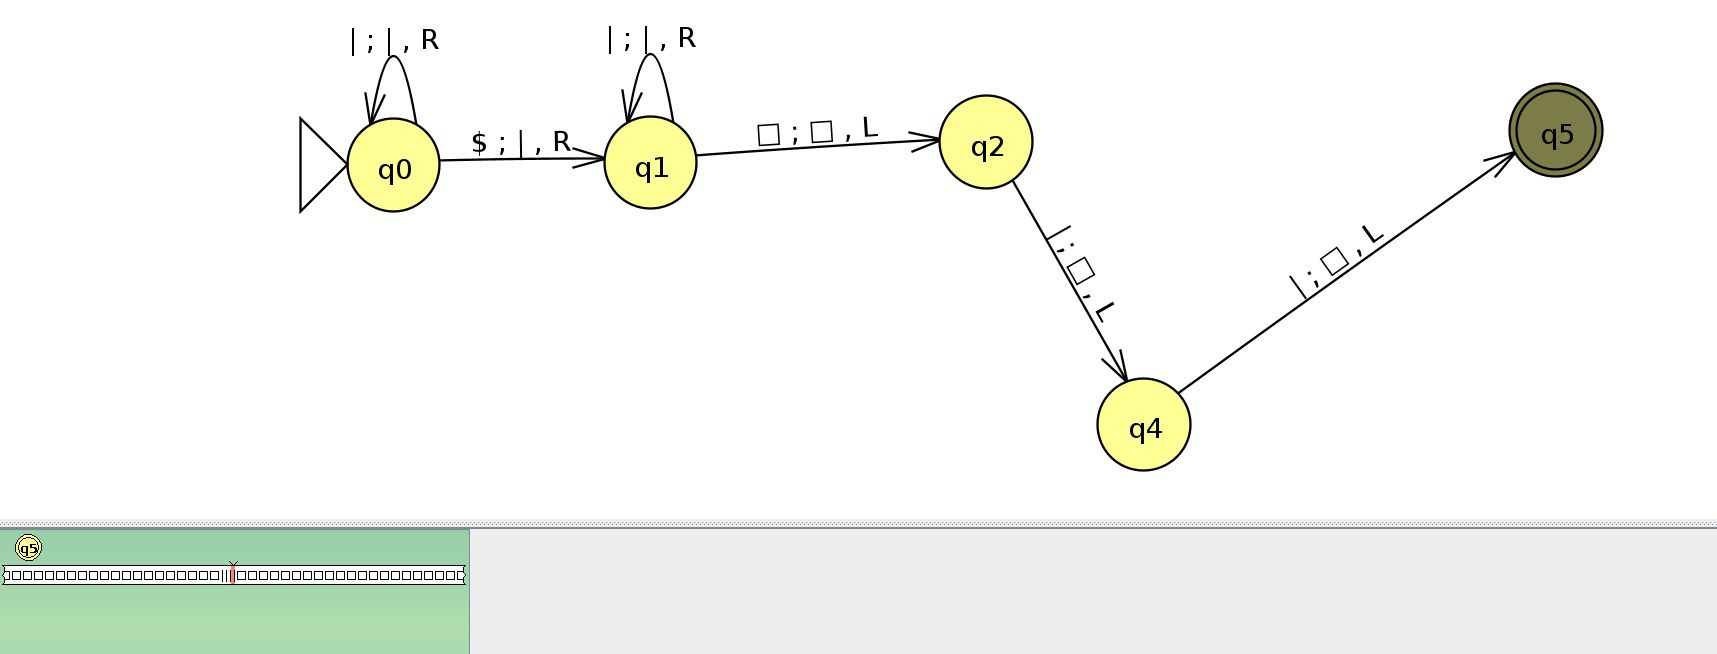
\includegraphics[scale=0.55]{TM_Ej1.jpg}


 
\newpage 

\section*{2. Define a recursive function for the sum of three values.}
Primero partimos de la suma de dos valores que la definimos de esta forma:
\begin{center}
    $suma({n,m})=\left\{ 
\begin{array}{ll}
\pi^1_{1} & \qquad \text{si m = 0}   \\
\sigma (\pi^3_{3}(n,m-1,suma({n,m-1}))) & \qquad \text {si m $>$ 0}
\end{array}\right.$
\end{center}

Siendo $\sigma$ la función recursiva sucesor:

$\sigma: \mathbb{N} \to \mathbb{N}$

$\sigma(n)=n+1$\\

Con esta podemos expresar la suma de tres valores:
\begin{center}
    $suma'({n,m,p})=\left\{ 
\begin{array}{ll}
suma({n,m-1}) & \qquad \text{si p = 0}   \\
\sigma (\pi^4_{4}(n,m,p-1,suma'({n,m,p-1}))) & \qquad \text {si p $>$ 0}
\end{array}\right.$
\end{center}

\newpage 
A continuación, podemos ver la ejecución de la función para los argumentos 3,5,2:

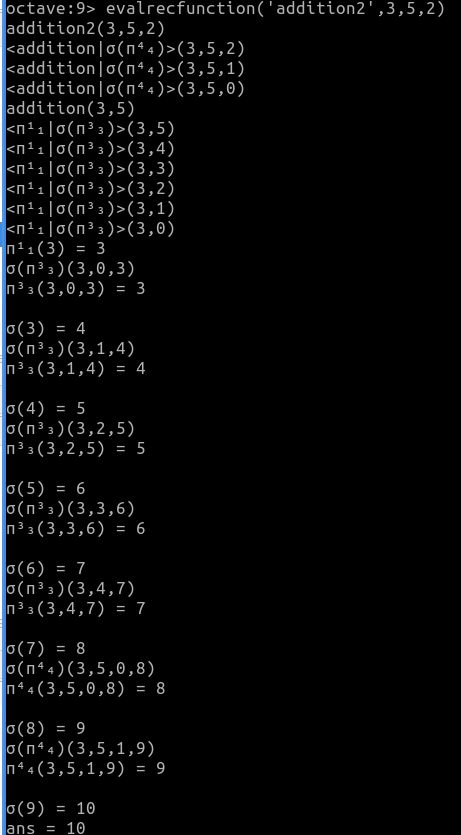
\includegraphics[scale=0.75]{suma'_Octave.jpg}


\section*{3. Implement a WHILE program that computes the sum of 3 values. You
must use an auxiliary variable that accumulates the result of the sum.}

\whileprogram{suma3arg}{3}{

}{s}

\begin{whilecode}[H]

  $X_4 \Assig X_1$\;
 \While{$X_2 \not = 0$}{

  $X_4 \Assig X_4 + 1$\;
  $X_2 \Assig X_2 - 1$\;
 }
 \While{$X_3 \not = 0$}{

  $X_4 \Assig X_4 + 1$\;
  $X_3 \Assig X_3 - 1$\;
 }
  $X_1 \Assig X_4$\;
\end{whilecode}

\newpage 


\end{document}